\documentclass[12pt]{article}

% ---- CeAI style (provides geometry, boxes, tikz, etc.) ----
\usepackage{ceai}

% ---- Additional packages ----
\usepackage{listings}
\usepackage{fontawesome5}
\usepackage{booktabs}
\usepackage{tabularx}
\usepackage{multicol}
\usepackage[super]{nth}

% ---- Listings style for bash / terminal ----
\lstdefinestyle{term}{
  basicstyle=\ttfamily\small,
  backgroundcolor=\color{gray!8},
  frame=single,
  framerule=0.4pt,
  rulecolor=\color{gray!60},
  breaklines=true,
  columns=fullflexible,
  showstringspaces=false,
  commentstyle=\color{green!50!black},
  morecomment=[l]{\#},
  xleftmargin=4pt,
  xrightmargin=4pt,
  aboveskip=8pt,
  belowskip=4pt,
}

% ---- Shortcuts ----
\newcommand{\cmd}[1]{\texttt{\$ #1}}
\newcommand{\key}[1]{\keystroke{#1}}
\newcommand{\keystroke}[1]{%
  \tikz[baseline=(key.base)]{%
    \node[draw, rounded corners=2pt, inner sep=2pt, fill=gray!10,
          font=\ttfamily\small] (key) {#1};%
  }%
}

% ---- Title ----
\title{\textbf{Tutorial 5: Getting Started with OpenCode}\\[4pt]
       {\large AI Coding Agent for the Terminal}}
\author{CE 488/5588 --- Applied Artificial Intelligence}
\date{Spring 2026}

\begin{document}
\maketitle

\begin{ch-box}
This tutorial walks you through installing \textbf{OpenCode} --- an AI coding agent that lives in your terminal --- and getting it ready for class.  By the end you will be able to chat with an AI that reads your code, edits files, runs commands, and more, all from the command line.

\medskip\noindent\textbf{What you will do today:}
\begin{enumerate}[nosep]
  \item Set up your Mac or Windows~PC for terminal work
  \item Install OpenCode
  \item Connect to an AI model (Google or OpenAI)
  \item Learn the key shortcuts every OpenCode user should know
  \item Set up safety rules so nothing gets deleted without your permission
\end{enumerate}
\end{ch-box}

% ===========================================================
\section{What Is OpenCode?}
% ===========================================================

OpenCode is a \emph{terminal-based} AI assistant.  Think of it as ChatGPT that can actually \emph{see your project} --- it reads your files, understands your codebase, edits code, runs tests, and even searches the web, all from inside your terminal~\cite{opencode2025,opencode_readme2025}.

\begin{def-box}
Unlike browser-based AI tools where you copy-paste code back and forth, OpenCode works \emph{inside} your project directory.  It sees what you see.  That makes it far more powerful --- and also why we need safety rules (Section~\ref{sec:safety}).
\end{def-box}

\begin{alert-box}
\textbf{Good to know:} The original OpenCode project was archived in September 2025 and is now maintained under an active distribution by AnomalyCo~\cite{anomalyco_opencode2026,opencode_install2026}.  This tutorial covers the \emph{current} version.
\end{alert-box}

% ===========================================================
\section{Setting Up Your Mac}
% ===========================================================

\begin{alert-box}
\textbf{On Windows?} Skip ahead to Section~\ref{sec:windows}.
\end{alert-box}

% ---- Flow chart: macOS setup ----
\begin{center}
\begin{tikzpicture}[
    node distance=1.4cm,
    every node/.style={align=center, font=\small},
    step/.style={rectangle, rounded corners=4pt, draw=blue!70!black,
                 fill=ceaiLightBlue, minimum width=5.2cm, minimum height=0.9cm},
    arr/.style={-{Stealth[length=6pt]}, thick, blue!70!black}
  ]
  \node[step] (brew)    {Install Homebrew\\(\texttt{brew})};
  \node[step, below=of brew]   (iterm)   {Install iTerm2\\+ CLI tools};
  \node[step, below=of iterm]  (oc)      {Install OpenCode\\(\texttt{curl \ldots\ | bash})};
  \node[step, below=of oc]     (verify)  {Verify:\\\texttt{opencode --version}};
  \draw[arr] (brew)  -- (iterm);
  \draw[arr] (iterm) -- (oc);
  \draw[arr] (oc)    -- (verify);
\end{tikzpicture}
\end{center}

% -----------------------------------------------------------
\subsection{Step 0 --- Install Homebrew}

Homebrew is the package manager for macOS --- it makes installing everything else a breeze.  Think of it as an app store for your terminal~\cite{homebrew2026}.

\begin{ex-box}
\textbf{If you already have Homebrew,} skip to Step~1.  If you are not sure, run:
\begin{lstlisting}[style=term]
brew --version
\end{lstlisting}
If that prints a version number you are good.  Otherwise, let us install it.
\end{ex-box}

Open \textbf{Terminal.app} (\key{Cmd}+\key{Space}, type \emph{Terminal}, press \key{Enter}) and paste:

\begin{lstlisting}[style=term]
/bin/bash -c "$(curl -fsSL https://raw.githubusercontent.com/Homebrew/install/HEAD/install.sh)"
\end{lstlisting}

\begin{alert-box}
\textbf{What happens next:}
\begin{itemize}[nosep]
  \item It will ask for your Mac password.  \textbf{Type it and press \key{Enter}} --- the characters will not show on screen (this is normal).
  \item The script runs for 5--10 minutes, installing Xcode Command Line Tools along the way.
  \item When it finishes it may print two lines starting with \texttt{echo} and \texttt{eval}.  \textbf{Copy and run those lines exactly as shown.}  On Apple~Silicon Macs they usually look like:
\end{itemize}
\end{alert-box}

\begin{lstlisting}[style=term]
echo 'eval "$(/opt/homebrew/bin/brew shellenv)"' >> ~/.zprofile
eval "$(/opt/homebrew/bin/brew shellenv)"
\end{lstlisting}

Now verify everything is working:

\begin{lstlisting}[style=term]
brew --version
brew doctor
\end{lstlisting}

\cmd{brew doctor} may show warnings --- that is usually fine.  Focus on anything that says \emph{Error} and ignore the rest.

% -----------------------------------------------------------
\subsection{Step 1 --- Install iTerm2 + Essentials}

macOS ships with a built-in Terminal, but iTerm2 is much better for running OpenCode.  It supports true color, smooth scrolling, and proper keyboard mappings~\cite{iterm2026}.

\begin{lstlisting}[style=term]
# iTerm2 -- a better terminal for macOS
brew install --cask iterm2
# A handful of CLI tools you will thank yourself for having
brew install git curl wget tree tmux
\end{lstlisting}

\begin{ex-box}
\textbf{Why these extras?}
\begin{description}[nosep, leftmargin=1.6cm]
  \item[\texttt{git}] Your safety net --- we set this up in Section~\ref{sec:safety}.
  \item[\texttt{curl}/\texttt{wget}] Downloading things from the internet.
  \item[\texttt{tree}] Visualising folder structures.
  \item[\texttt{tmux}] Keeping terminal sessions alive if you disconnect.
\end{description}
\end{ex-box}

After installation, \textbf{launch iTerm2} from Spotlight (\key{Cmd}+\key{Space} $\to$ type \emph{iTerm}).  Use iTerm2 for everything from here on.

% -----------------------------------------------------------
\subsection{Step 2 --- Install OpenCode}

In iTerm2, run:

\begin{lstlisting}[style=term]
curl -fsSL https://opencode.ai/install | bash
\end{lstlisting}

That is it!  The script will:
\begin{itemize}[nosep]
  \item[\faCheckCircle] Detect your Mac's chip (Intel or Apple~Silicon) automatically.
  \item[\faCheckCircle] Download OpenCode to \texttt{\textasciitilde/.opencode/bin/}.
  \item[\faCheckCircle] Add it to your \texttt{PATH} so you can run it from anywhere~\cite{opencode_install2026}.
\end{itemize}

% -----------------------------------------------------------
\subsection{Step 3 --- Verify}

Open a \textbf{new} iTerm2 tab (or run \cmd{source \textasciitilde/.zshrc}) and check:

\begin{lstlisting}[style=term]
opencode --version
\end{lstlisting}

You should see something like \texttt{1.14.30} or newer.  If you see a version number, you are all set!

\begin{ex-box}
\textbf{Alternative:} You can also install via Homebrew:
\begin{lstlisting}[style=term]
brew install opencode-ai/tap/opencode
\end{lstlisting}
\end{ex-box}

% ===========================================================
\section{Setting Up Your Windows PC}
\label{sec:windows}
% ===========================================================

Windows needs a Linux layer called \textbf{WSL~2} to run OpenCode.  Do not worry --- it is just a few commands.

\begin{center}
\begin{tikzpicture}[
    node distance=1.4cm,
    every node/.style={align=center, font=\small},
    step/.style={rectangle, rounded corners=4pt, draw=blue!70!black,
                 fill=ceaiLightBlue, minimum width=5.2cm, minimum height=0.9cm},
    arr/.style={-{Stealth[length=6pt]}, thick, blue!70!black}
  ]
  \node[step] (wsl)    {Enable WSL~2\\(\texttt{wsl --install})};
  \node[step, below=of wsl]   (wterm)   {Install Windows\\Terminal};
  \node[step, below=of wterm]  (woc)    {Install OpenCode\\(\texttt{curl \ldots\ | bash})};
  \node[step, below=of woc]    (wver)   {Verify:\\\texttt{opencode --version}};
  \draw[arr] (wsl)  -- (wterm);
  \draw[arr] (wterm) -- (woc);
  \draw[arr] (woc)   -- (wver);
\end{tikzpicture}
\end{center}

% -----------------------------------------------------------
\subsection{Step 1 --- Enable WSL~2}

Open \textbf{PowerShell as Administrator} (right-click PowerShell $\to$ \emph{Run as Administrator}) and run~\cite{microsoft_wsl2026}:

\begin{lstlisting}[style=term]
wsl --install
\end{lstlisting}

Restart your computer when prompted.  This installs Ubuntu as your Linux environment.

% -----------------------------------------------------------
\subsection{Step 2 --- Install Windows Terminal}

Windows Terminal is much better than the old Command Prompt --- it supports proper colors, Unicode, and keyboard input.

\begin{lstlisting}[style=term]
winget install Microsoft.WindowsTerminal
\end{lstlisting}

% -----------------------------------------------------------
\subsection{Step 3 --- Install OpenCode}

Open \textbf{Windows Terminal}, start an \textbf{Ubuntu} tab, and run:

\begin{lstlisting}[style=term]
curl -fsSL https://opencode.ai/install | bash
\end{lstlisting}

% -----------------------------------------------------------
\subsection{Step 4 --- Verify}

\begin{lstlisting}[style=term]
opencode --version
\end{lstlisting}

\begin{alert-box}
If \texttt{opencode} is not found, reload your shell:
\begin{lstlisting}[style=term]
source ~/.bashrc    # or source ~/.zshrc if you use Zsh
\end{lstlisting}
Or manually add to your \texttt{PATH}:
\begin{lstlisting}[style=term]
export PATH="$HOME/.opencode/bin:$PATH"
\end{lstlisting}
\end{alert-box}

% ===========================================================
\section{Connecting to an AI Model}
\label{sec:connect}
% ===========================================================

OpenCode needs access to an AI model to think.  There are \textbf{two ways} to connect:

\begin{center}
\begin{tikzpicture}[
    node distance=0.6cm and 2.5cm,
    every node/.style={align=center, font=\small},
    opt/.style={rectangle, rounded corners=6pt, draw=blue!70!black,
                minimum width=5.5cm, minimum height=1.8cm},
    arr/.style={-{Stealth[length=6pt]}, thick, blue!70!black}
  ]

  \node[opt, fill=ceaiLightBlue] (oauth)
    {\textbf{Option A: OAuth Login}\\(Recommended \faStar)\\
     Sign in with Google/OpenAI account\\
     like logging into a website};

  \node[opt, right=of oauth, fill=white] (api)
    {\textbf{Option B: Manual API Key}\\ Paste a key string\\
     into your shell config};

  \node[above=0.5cm of oauth, font=\bfseries] (start) {Choose your method};

  \draw[arr] (start.south) -- ++(0,-0.2) -| (oauth.north);
  \draw[arr] (start.south) -- ++(0,-0.2) -| (api.north);

\end{tikzpicture}
\end{center}

\begin{def-box}
\textbf{We recommend OAuth for this course.}  It is simpler, safer (no keys to leak), and works with free-tier accounts.
\end{def-box}

% ---- Flow chart: OAuth login ----
\begin{center}
\begin{tikzpicture}[
    node distance=1.2cm,
    every node/.style={align=center, font=\small},
    step/.style={rectangle, rounded corners=4pt, draw=blue!70!black,
                 fill=ceaiLightBlue, minimum width=5.8cm, minimum height=0.85cm},
    arr/.style={-{Stealth[length=6pt]}, thick, blue!70!black}
  ]
  \node[step] (cd)   {\texttt{cd \textasciitilde/my-project \&\& opencode}};
  \node[step, below=of cd]   (auth)  {Run \texttt{opencode providers login -p openai}\\or \texttt{-p google}};
  \node[step, below=of auth] (signin){Sign in via browser (OpenAI)\\or paste API key (Google)};
  \node[step, below=of signin](verify){\texttt{opencode providers list}\\(check green dot)};
  \node[step, below=of verify](model) {Press \key{Ctrl+O} $\to$ pick a model};
  \draw[arr] (cd)     -- (auth);
  \draw[arr] (auth)   -- (signin);
  \draw[arr] (signin) -- (verify);
  \draw[arr] (verify) -- (model);
\end{tikzpicture}
\end{center}

% -----------------------------------------------------------
\subsection{Option A --- OAuth Login (Recommended)}

This works just like signing into a website --- no API key strings, no config file editing.

\subsubsection*{Step 1 --- Open a project}

\begin{lstlisting}[style=term]
cd ~/my-project
opencode
\end{lstlisting}

\subsubsection*{Step 2 --- Sign in to a provider}

You can authenticate from your terminal (before or after launching OpenCode):

\begin{lstlisting}[style=term]
# OpenAI -- opens a browser for you to sign in
opencode providers login -p openai
\end{lstlisting}

\begin{lstlisting}[style=term]
# Google -- asks for your Gemini API key
opencode providers login -p google
\end{lstlisting}

For \textbf{OpenAI}, you will see a menu like:

\begin{lstlisting}[style=term]
  Add credential

  Login method
  * ChatGPT Pro/Plus (browser)      <- Pick this one!
    ChatGPT Pro/Plus (headless)
    Manually enter API Key
\end{lstlisting}

Choose \textbf{ChatGPT Pro/Plus (browser)} --- your web browser opens, you sign in to your ChatGPT account, and that is it.  Your terminal confirms:

\begin{lstlisting}[style=term]
  OpenAI credential saved
\end{lstlisting}

For \textbf{Google}, you will need a Gemini API key.  Get one free at \url{https://aistudio.google.com/apikey}~\cite{google_aistudio2026}.  Copy the key and paste it when prompted.

\subsubsection*{Step 3 --- Double-check your login}

\begin{lstlisting}[style=term]
opencode providers list
\end{lstlisting}

You should see something like:

\begin{lstlisting}[style=term]
  Credentials

  * OpenAI    oauth      <- You are in!
  * Google    api        <- Key configured
\end{lstlisting}

The green dot \texttt{*} means the credential is active and working.

\subsubsection*{Step 4 --- Pick a model}

Inside the OpenCode TUI, press \key{Ctrl+O} to open the \textbf{model picker}.  Use arrow keys to browse and press \key{Enter} to select.

\begin{ex-box}
\textbf{Recommended models for this course:}

\medskip
\begin{tabular}{lll}
\toprule
\textbf{Provider} & \textbf{Model} & \textbf{Why?} \\
\midrule
OpenAI & \texttt{gpt-5.2}         & Strongest general-purpose model \\
OpenAI & \texttt{gpt-5.1-codex}   & Built for code tasks \\
Google & \texttt{gemini-2.5-flash} & Fast, generous free tier \\
Google & \texttt{gemini-2.5-pro}   & More capable, higher limits \\
\bottomrule
\end{tabular}

\medskip
\textbf{No account?} OpenCode ships with free models that need zero setup.  Look for names ending in \texttt{-free} (like \texttt{opencode/hy3-preview-free}).  Perfect for trying things out.
\end{ex-box}

% -----------------------------------------------------------
\subsection{Option B --- Manual API Keys (Alternative)}

If you prefer managing keys yourself, or if you are on a headless server without a browser, add these lines to \texttt{\textasciitilde/.zshrc} (Mac) or \texttt{\textasciitilde/.bashrc} (WSL/Linux):

\begin{lstlisting}[style=term]
export ANTHROPIC_API_KEY="sk-ant-..."     # Claude models
export OPENAI_API_KEY="sk-..."            # GPT models
export GEMINI_API_KEY="..."               # Gemini models
\end{lstlisting}

Then reload:

\begin{lstlisting}[style=term]
source ~/.zshrc     # Mac
source ~/.bashrc    # WSL/Linux
\end{lstlisting}

\begin{alert-box}
\textbf{Never commit API keys to Git.} Add \texttt{.env} files to your \texttt{.gitignore}.
\end{alert-box}

% -----------------------------------------------------------
\subsection{Configuration Files}

OpenCode reads config from these locations (highest priority first)~\cite{opencode_readme2025}:

\begin{center}
\begin{tabular}{cll}
\toprule
\textbf{Priority} & \textbf{Location} & \textbf{Scope} \\
\midrule
1st & \texttt{./.opencode.json} & Project-local \\
2nd & \texttt{\textasciitilde/.config/opencode/opencode.json} & User defaults \\
\bottomrule
\end{tabular}
\end{center}

\begin{ex-box}
\textbf{For this course}, your instructor will provide the config file.  Just paste it into \texttt{\textasciitilde/.config/opencode/opencode.json}.
\end{ex-box}

% ===========================================================
\section{Using OpenCode}
% ===========================================================

\subsection{Starting a Session}

Navigate to your project and launch:

\begin{lstlisting}[style=term]
cd ~/my-project
opencode
\end{lstlisting}

You will see the TUI --- a full-screen terminal interface with a message box at the bottom.  That is where you type your prompts.

\subsection{Handy CLI Commands}

\begin{center}
\begin{tabular}{ll}
\toprule
\textbf{Command} & \textbf{What it does} \\
\midrule
\texttt{opencode}                        & Start the TUI in the current folder \\
\texttt{opencode -c /path/to/project}    & Start in a specific folder \\
\texttt{opencode -p "explain this code"} & Ask one question, get an answer, exit \\
\texttt{opencode -p "do X" -f json}     & Same, but output as JSON \\
\texttt{opencode -p "do X" -q}           & Same, but quiet (no spinner) \\
\texttt{opencode -c}                     & Continue your last session \\
\texttt{opencode --version}              & Check the version \\
\texttt{opencode -h}                     & Show all options \\
\bottomrule
\end{tabular}
\end{center}

\subsection{Keyboard Shortcuts Every User Should Know}

\begin{center}
\begin{tabular}{ll}
\toprule
\textbf{Shortcut} & \textbf{What it does} \\
\midrule
\key{i}           & Start typing a message \\
\key{Ctrl+S}      & Send your message \\
\key{Ctrl+O}      & Switch AI model \\
\key{Ctrl+K}      & Open the command palette \\
\key{Ctrl+N}      & New session \\
\key{Ctrl+A}      & Switch between sessions \\
\key{Ctrl+C}      & Quit OpenCode \\
\key{Esc}          & Close any dialog \\
\bottomrule
\end{tabular}
\end{center}

% ---- Permission flow diagram ----
\subsection{Permission Keys --- When OpenCode Asks ``Can I do this?''}

\begin{center}
\begin{tikzpicture}[
    node distance=1.0cm,
    every node/.style={align=center, font=\small},
    act/.style={rectangle, rounded corners=4pt, draw=blue!70!black,
                fill=ceaiLightBlue, minimum width=4.5cm, minimum height=0.8cm},
    dec/.style={diamond, draw=orange!80!black, fill=ceaiAlertYellow,
                minimum width=2.8cm, minimum height=1.6cm, inner sep=1pt,
                font=\small},
    ok/.style={rectangle, rounded corners=4pt, draw=green!60!black,
               fill=green!10, minimum width=3.2cm, minimum height=0.8cm},
    no/.style={rectangle, rounded corners=4pt, draw=red!70!black,
               fill=red!10, minimum width=3.2cm, minimum height=0.8cm},
    arr/.style={-{Stealth[length=6pt]}, thick}
  ]

  \node[act] (req) {OpenCode wants\\to act (edit, run, delete)};

  \node[dec, below=of req] (perm) {Review \\the action};

  \node[ok, below left=1cm and 1.2cm of perm]  (a) {\key{a} --- Allow once};
  \node[ok, below=1cm of perm]                 (A) {\key{A} --- Allow session};
  \node[no, below right=1cm and 1.2cm of perm] (d) {\key{d} --- Deny};

  \draw[arr] (req) -- (perm);
  \draw[arr] (perm) -- (a);
  \draw[arr] (perm) -- (A);
  \draw[arr] (perm) -- (d);
\end{tikzpicture}
\end{center}

% ===========================================================
\section{Safety Rules --- Do Not Skip This!}
\label{sec:safety}
% ===========================================================

\begin{alert-box}
OpenCode is powerful.  It can read, write, \emph{and delete} your files.  It can run shell commands on your machine.  \textbf{It always asks for your permission first}~\cite{opencode_readme2025,opencode_permission2025} --- but \emph{you} need to know what to approve and what to reject.
\end{alert-box}

Whenever OpenCode wants to do something --- edit a file, run a command, delete something --- it pauses and shows you a \textbf{permission prompt}.  You review what it wants to do, then press \key{a} (allow once), \key{A} (allow all for this session), or \key{d} (deny).

% -----------------------------------------------------------
\subsection{Mandatory Safety Policies for This Course}

\begin{alert-box}
\textbf{Rule 1:} Never press \key{A} (Allow Session) for anything that \emph{writes} or \emph{deletes}.  Only use \key{A} for read-only tools like \texttt{view}, \texttt{glob}, and \texttt{grep}.  For \texttt{bash}, \texttt{edit}, and \texttt{write}, always use \key{a} (allow once) so you can review each action individually.
\end{alert-box}

\begin{alert-box}
\textbf{Rule 2:} Read the full command before approving.  If OpenCode proposes a command containing \texttt{rm}, \texttt{del}, \texttt{drop}, \texttt{truncate}, or \texttt{format}, verify the target path carefully.
\end{alert-box}

\begin{alert-box}
\textbf{Rule 3:} Read the diff before approving edits.  OpenCode shows you exactly what it is about to change.  Take 5 seconds to glance at it.
\end{alert-box}

\begin{alert-box}
\textbf{Rule 4:} If you do not understand a command, press \key{d} to deny it.  Then ask OpenCode to explain what the command would have done.  No shame in being cautious.
\end{alert-box}

\begin{alert-box}
\textbf{Rule 5:} Always use Git as your safety net.  Before every OpenCode session:
\begin{lstlisting}[style=term]
git init                    # (first time only)
git add -A
git commit -m "Snapshot before AI session"
\end{lstlisting}
If OpenCode makes a change you do not like, you can always undo it:
\begin{lstlisting}[style=term]
git restore .               # Undo all uncommitted changes
git checkout HEAD -- file.py # Undo changes to a specific file
\end{lstlisting}
\end{alert-box}

\begin{alert-box}
\textbf{Rule 6:} Keep secrets out of your project files.  OpenCode reads everything in your project directory.  Add \texttt{.env} files to \texttt{.gitignore} and never ask the agent to read them.
\end{alert-box}

\subsection{About Auto-Approval}

OpenCode has a non-interactive mode (\texttt{-p}) that auto-approves \emph{everything}~\cite{opencode_readme2025}:

\begin{lstlisting}[style=term]
# WARNING: AUTO-APPROVES ALL ACTIONS -- be careful!
opencode -p "refactor the utils module"
\end{lstlisting}

\begin{def-box}
This mode is great for scripts, but \textbf{do not use it interactively} unless you have committed your current work to Git first.
\end{def-box}

% ===========================================================
\section{Things to Try}
% ===========================================================

Now that OpenCode is set up, here are some things to try:

\begin{ex-box}
\textbf{Ask a question:}  Type this in the message box and press \key{Ctrl+S}:
\begin{lstlisting}[style=term,frame=none,backgroundcolor=\color{white}]
What does the function calculate_loss() in train.py do?
\end{lstlisting}
OpenCode will find and read the file, then explain it.
\end{ex-box}

\begin{ex-box}
\textbf{Ask it to edit code:}
\begin{lstlisting}[style=term,frame=none,backgroundcolor=\color{white}]
Add type hints to all functions in utils.py
\end{lstlisting}
It will propose edits.  Review the diff and press \key{a} to approve or \key{d} to deny.
\end{ex-box}

\begin{ex-box}
\textbf{Ask it to run tests:}
\begin{lstlisting}[style=term,frame=none,backgroundcolor=\color{white}]
Run the test suite and report any failures
\end{lstlisting}
It will propose a command like \texttt{pytest tests/ -v}.  Review the command, then approve.
\end{ex-box}

\begin{ex-box}
\textbf{Search your codebase:}
\begin{lstlisting}[style=term,frame=none,backgroundcolor=\color{white}]
Find all Python files that import numpy
\end{lstlisting}
\end{ex-box}

\begin{ex-box}
\textbf{Switch models on the fly:}  Press \key{Ctrl+O} to pick a different model.  Try a free model first, then switch to something more powerful.

\textbf{Manage sessions:}
\begin{itemize}[nosep]
  \item \key{Ctrl+N} --- start a fresh conversation
  \item \key{Ctrl+A} --- jump between sessions
  \item Conversations are saved automatically in a local database~\cite{opencode_readme2025}
\end{itemize}
\end{ex-box}

% ===========================================================
\section{Uninstalling}
% ===========================================================

If you ever need to remove OpenCode:

\begin{lstlisting}[style=term]
opencode uninstall
\end{lstlisting}

Or manually:

\begin{lstlisting}[style=term]
rm -rf ~/.opencode/bin/opencode
# Then remove the PATH line from ~/.zshrc or ~/.bashrc
\end{lstlisting}

% ===========================================================
\section{Quick Reference Card}
% ===========================================================

\begin{center}
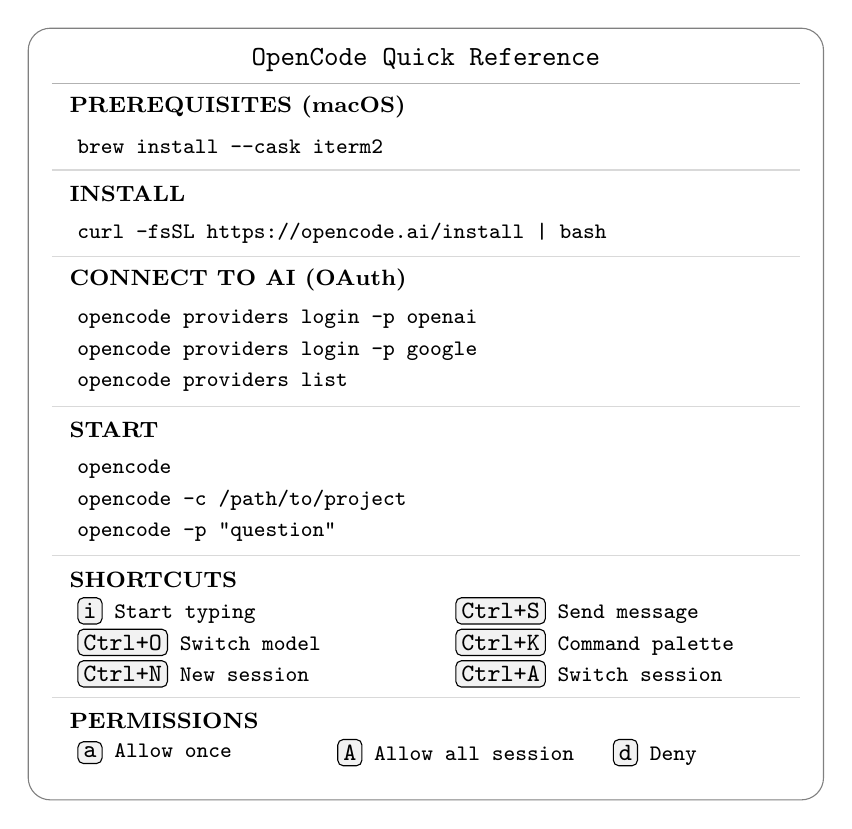
\begin{tikzpicture}[
    every node/.style={font=\footnotesize\ttfamily, anchor=west},
    btnode/.style={draw, rounded corners=2pt, fill=ceaiLightBlue,
                   inner sep=3pt, font=\footnotesize\ttfamily}
  ]
  % Background
  \fill[white, draw=black!50, rounded corners=8pt]
    (-0.3,-0.3) rectangle (9.8,9.5);

  % Title
  \node[font=\bfseries\normalsize\ttfamily, anchor=center] at (4.75,9.1)
    {OpenCode Quick Reference};

  \draw[black!30] (0,8.8) -- (9.5,8.8);

  % PREREQUISITES
  \node[font=\footnotesize\bfseries] at (0.1,8.5) {PREREQUISITES (macOS)};
  \node at (0.2,8.0) {brew install --cask iterm2};

  \draw[black!15] (0,7.7) -- (9.5,7.7);

  % INSTALL
  \node[font=\footnotesize\bfseries] at (0.1,7.4) {INSTALL};
  \node at (0.2,6.9) {curl -fsSL https://opencode.ai/install | bash};

  \draw[black!15] (0,6.6) -- (9.5,6.6);

  % AUTH
  \node[font=\footnotesize\bfseries] at (0.1,6.3) {CONNECT TO AI (OAuth)};
  \node at (0.2,5.8) {opencode providers login -p openai};
  \node at (0.2,5.4) {opencode providers login -p google};
  \node at (0.2,5.0) {opencode providers list};

  \draw[black!15] (0,4.7) -- (9.5,4.7);

  % START
  \node[font=\footnotesize\bfseries] at (0.1,4.4) {START};
  \node at (0.2,3.9) {opencode};
  \node at (0.2,3.5) {opencode -c /path/to/project};
  \node at (0.2,3.1) {opencode -p "question"};

  \draw[black!15] (0,2.8) -- (9.5,2.8);

  % SHORTCUTS (two columns)
  \node[font=\footnotesize\bfseries] at (0.1,2.5) {SHORTCUTS};
  \node at (0.2,2.1) {\key{i} Start typing};
  \node at (5.0,2.1) {\key{Ctrl+S} Send message};
  \node at (0.2,1.7) {\key{Ctrl+O} Switch model};
  \node at (5.0,1.7) {\key{Ctrl+K} Command palette};
  \node at (0.2,1.3) {\key{Ctrl+N} New session};
  \node at (5.0,1.3) {\key{Ctrl+A} Switch session};

  \draw[black!15] (0,1.0) -- (9.5,1.0);

  % PERMISSIONS
  \node[font=\footnotesize\bfseries] at (0.1,0.7) {PERMISSIONS};
  \node at (0.2,0.3) {\key{a} Allow once};
  \node at (3.5,0.3) {\key{A} Allow all session};
  \node at (7.0,0.3) {\key{d} Deny};
\end{tikzpicture}
\end{center}

% ===========================================================
% References
% ===========================================================

\begin{thebibliography}{9}

\bibitem{opencode2025}
opencode-ai, ``OpenCode: A powerful AI coding agent. Built for the terminal,'' \emph{GitHub}, 2025. Available: \url{https://github.com/opencode-ai/opencode}

\bibitem{opencode_readme2025}
opencode-ai, ``OpenCode README --- Configuration, Usage, and Keyboard Shortcuts,'' \emph{GitHub}, 2025. Available: \url{https://github.com/opencode-ai/opencode/blob/main/README.md}

\bibitem{anomalyco_opencode2026}
anomalyco, ``OpenCode (active distribution),'' \emph{GitHub}, 2026. Available: \url{https://github.com/anomalyco/opencode}

\bibitem{opencode_install2026}
OpenCode, ``Install script,'' \emph{opencode.ai}, 2026. Available: \url{https://opencode.ai/install}

\bibitem{iterm2026}
G.~Nachman, ``iTerm2 --- macOS Terminal Replacement,'' \emph{iterm2.com}, 2026. Available: \url{https://iterm2.com}

\bibitem{microsoft_wsl2026}
Microsoft, ``Windows Subsystem for Linux Documentation,'' \emph{Microsoft Learn}, 2026. Available: \url{https://learn.microsoft.com/en-us/windows/wsl/}

\bibitem{opencode_permission2025}
opencode-ai, ``Permission system: \texttt{internal/permission/permission.go} and \texttt{internal/tui/components/dialog/permission.go},'' \emph{GitHub}, 2025. Available: \url{https://github.com/opencode-ai/opencode/blob/main/internal/permission/permission.go}

\bibitem{homebrew2026}
M.~Howell and Homebrew Contributors, ``Homebrew --- The Missing Package Manager for macOS (or Linux),'' \emph{brew.sh}, 2026. Available: \url{https://brew.sh}

\bibitem{google_aistudio2026}
Google, ``Google AI Studio --- Get an API Key,'' \emph{aistudio.google.com}, 2026. Available: \url{https://aistudio.google.com/apikey}

\end{thebibliography}

\end{document}